\documentclass[12pt,-letter paper]{article}
\usepackage{siunitx}
\usepackage{setspace}
\usepackage{gensymb}
\usepackage{xcolor}
\usepackage{caption}
%\usepackage{subcaption}
\doublespacing
\singlespacing
\usepackage[none]{hyphenat}
\usepackage{amssymb}
\usepackage{relsize}
\usepackage[cmex10]{amsmath}
\usepackage{mathtools}
\usepackage{amsmath}
\usepackage{commath}
\usepackage{amsthm}
\interdisplaylinepenalty=2500
%\savesymbol{iint}
\usepackage{txfonts}
%\restoresymbol{TXF}{iint}
\usepackage{wasysym}
\usepackage{amsthm}
\usepackage{mathrsfs}
\usepackage{txfonts}
\let\vec\mathbf{}
\usepackage{stfloats}
\usepackage{float}
\usepackage{cite}
\usepackage{cases}
\usepackage{subfig}
%\usepackage{xtab}
\usepackage{longtable}
\usepackage{multirow}
%\usepackage{algorithm}
\usepackage{amssymb}
%\usepackage{algpseudocode}
\usepackage{enumitem}
\usepackage{mathtools}
%\usepackage{eenrc}
%\usepackage[framemethod=tikz]{mdframed}
\usepackage{listings}
%\usepackage{listings}
\usepackage[latin1]{inputenc}
%%\usepackage{color}{   
%%\usepackage{lscape}
\usepackage{textcomp}
\usepackage{titling}
\usepackage{hyperref}
%\usepackage{fulbigskip}   
\usepackage{tikz}
\usepackage{graphicx}
\lstset{
  frame=single,
  breaklines=true
}
\let\vec\mathbf{}
\usepackage{enumitem}
\usepackage{graphicx}
\usepackage{siunitx}
\let\vec\mathbf{}
\usepackage{enumitem}
\usepackage{graphicx}
\usepackage{enumitem}
\usepackage{tfrupee}
\usepackage{amsmath}
\usepackage{amssymb}
\usepackage{mwe} % for blindtext and example-image-a in example
\usepackage{wrapfig}
\graphicspath{{figs/}}
\providecommand{\cbrak}[1]{\ensuremath{\left\{#1\right\}}}
\providecommand{\brak}[1]{\ensuremath{\left(#1\right)}}
%\providecommand{\norm}[1]{\left\lVert#1\right\rVert}
\newcommand{\myvec}[1]{\ensuremath{\begin{pmatrix}#1\end{pmatrix}}}
\newcommand{\augvec}[3]{\ensuremath{\begin{amatrix}{#1|#2}#3\end{amatrix}}}
\newcommand{\mydet}[1]{\ensuremath{\begin{vmatrix}#1\end{vmatrix}}}
\usepackage{subfig}\graphicspath{{/storage/self/primary/Download/latexnew/fig}}

%\newcommand{\abs}[1]{\lvert#1\rvert}
%\newcommand{\norm}[1]{\lVert#1\rVert}
\providecommand{\sbrak}[1]{\ensuremath{{}\left[#1\right]}}
\providecommand{\brak}[1]{\ensuremath{\left(#1\right)}}
\providecommand{\cbrak}[1]{\ensuremath{\left\{#1\right\}}}
%\newcommand{\myvec}[1]{\ensuremath{\begin{pmatrix}#1%\end{pmatrix}}}
\newcommand{\myaugvec}[2]{\ensuremath{\begin{amatrix}{#1}#2\end{amatrix}}}
%\newcommand{\mydet}[1]{\ensuremath{\begin{vmatrix}#1%\end{vmatrix}}}

\begin{document}
\title{\textbf{MATH-COMPUTING}}
\maketitle
\begin{enumerate}
 
    \item \textbf{Question(MATH-12.10.5.17):}
       Let $\vec{a}$ and $\vec{b}$ be two unit vectors and $\theta$ is the angle between them. Then $\vec{a}+\vec{b}$ is a unit vector.
    
 \begin{enumerate}[label=(\Alph*)]                     
 \item $\theta$=$\frac{\pi}{4}$
 \item $\theta$=$\frac{\pi}{3}$
  \item $\theta$=$\frac{\pi}{2}$
   \item $\theta$=$\frac{2\pi}{3}$
   \end{enumerate}

 \textbf{solution:}

Given,
\begin{align}
	\norm{\vec{a}} = \norm{\vec{b}}=1\\
	\norm{\vec{a}+\vec{b}}=1
\end{align}
Squaring on both sides, we get
\begin{align}
	\norm{\vec{a}+\vec{b}}^2=1^2
\\	
	\implies \norm{\vec{a}}^2 + \norm{\vec{b}}^2 + 2\vec{a}^{\top}\vec{b} = 1
\end{align}
Substituting eq (4) in eq (1), we get
\\
\begin{align}
	\implies 1+1+2(\norm{\vec{a}}\norm{\vec{b}}\cos{\theta})=1
	\\
	\implies 2+2(\norm{\vec{a}}\norm{\vec{b}}\cos{\theta})=1
        \\
	\implies 2(\norm{\vec{a}}\norm{\vec{b}}\cos{\theta})=-1
	\\
	\implies (\norm{\vec{a}}\norm{\vec{b}}\cos{\theta})=\frac{-1}{2}\label{eq:12/10/5/17/4}
\end{align}
Subtituting eq (1) in eq (8), we get
\begin{align}
	\implies \cos{\theta}=\frac{-1}{2}
	\\
	\implies \theta=\frac{2\pi}{3}
\end{align}
Assuming the co-ordinates:\\
  \begin{align}
{A}=\myvec{-2.31 \\ 3.98},\,
{B}=\myvec{0\\0},\,
{c}=\myvec{1.69\\0}\\
  \end{align}
To find angle B in a triangle ABC:\\
  \begin{align}
\cos{B} \triangleq \frac{(\vec{A}-\vec{B})^\top(\vec{C}-\vec{B})}{\norm{\vec{A}-\vec{B}}\norm{\vec{C}-\vec{B}}}\\
  \end{align}
  \begin{align} 
\vec{A} - \vec{B} = \myvec{-2.31 \\ 3.98}-\myvec{0 \\ 0} = \myvec{ -2.31\\ 3.98 }
 \end{align}

  \begin{align}
\vec{C} - \vec{B} = \myvec{1.69 \\ 0}-\myvec{0 \\ 0} = \myvec{ 1.69\\ 0 }\\
 \end{align}
  \begin{align}
\norm{\vec{A}-\vec{B}} \triangleq \sqrt{\brak{\vec{A}-\vec{B}}^{\top}\brak{\vec{A}-\vec{B}}} = \sqrt{\brak{{-2.31}-{3.98}}{\myvec{-2.31\\3.98}}} = 4.60\\
 \end{align}
  \begin{align}
\norm{\vec{C}-\vec{B}} \triangleq \sqrt{\brak{\vec{C}-\vec{B}}^{\top}\brak{\vec{C}-\vec{B}}} = \sqrt{\brak{{1.69}-{0}}{\myvec{1.69\\0}}} = 1.69\\
  \end{align}
Therefore:\\
 \begin{align}
\cos{B}=\frac{\brak{{-2.31}-{3.98}}{\myvec{1.69\\0}}}{\brak{4.60}\brak{1.69}} = \frac{-3.903}{7.774} = {0.501}\\
 \end{align}
  \begin{align}
 {B}=\cos^{-1}\brak{0.5} = 120^\degree
 \end{align}
 \begin{figure}[!h]
        \centering
        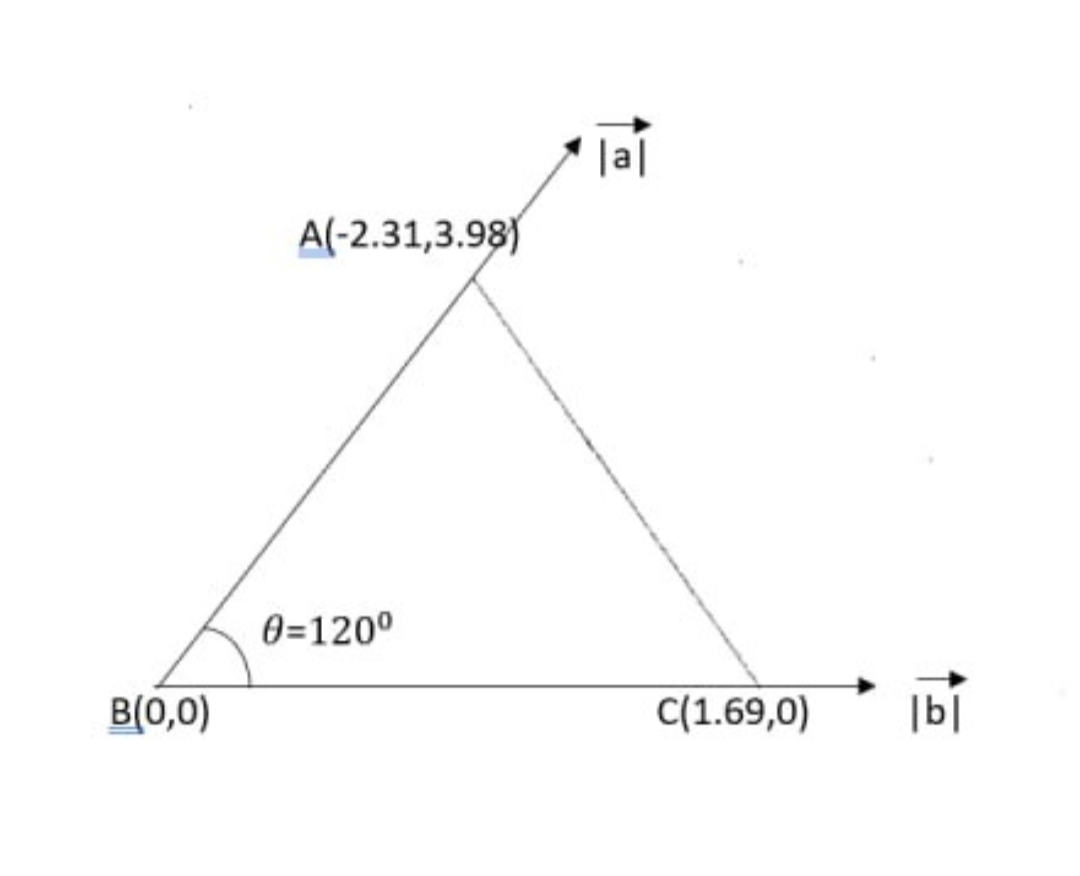
\includegraphics[width=\columnwidth]{math.jpeg}
        \caption{vectors}
        \label{fig:figure}
    \end{figure}
    
  \end{enumerate}
\end{document}y
